\documentclass[journal]{IEEEtran}
\usepackage{amsmath,amssymb}
\usepackage{booktabs}
\usepackage{graphicx}
\usepackage{hyperref}
\usepackage{multirow}

% ---- Anonymization toggle (paper-1 convention) ----
\newif\ifanonymous
\anonymoustrue

\ifanonymous
\newcommand{\repourl}{\url{https://anonymous.4open.science/status/moba-draft-policies}}
\newcommand{\deployurl}{\url{https://draft-assistant-review.vercel.app}}
\else
\newcommand{\repourl}{\url{https://github.com/maxsegan/moba-draft-policies}}
\newcommand{\deployurl}{\url{https://www.hotsfever.com}}
\fi
% ---- Pre-registration (OSF 3cxvd, registered 2026-09-27, embargoed to 2027) ----
\newcommand{\preregdate}{September 27, 2026}
\ifanonymous
\newcommand{\prereglink}{\url{https://osf.io/3cxvd/overview?view_only=dbe817f56afe4507865e44bf24510748}}
\else
\newcommand{\prereglink}{\url{https://osf.io/3cxvd}}
\fi
% ---------------------------------------------------

% ==== Arm names as macros: "frozen" is never written bare. ====
\newcommand{\maintained}{\textsc{maintained}}          % cumulative-refresh agent
\newcommand{\maintainedpred}{\textsc{maintained-d90}}  % decayed-aggregate stats (prediction champion)
\newcommand{\stalefour}{\textsc{unmaintained}}
\newcommand{\staleone}{\textsc{stale-1yr}}
\newcommand{\staletwo}{\textsc{stale-2yr}}
\newcommand{\leakyfrozen}{\textsc{leaky-frozen}}
% ==============================================================

\begin{document}

\title{Maintaining Draft Policies Under Meta Drift:\\ Data-Side Refresh Beats Retraining}
\ifanonymous
\author{Anonymous Authors}
\else
\author{Max~Segan and Hod~Lipson}
\fi
\maketitle

\begin{abstract}
Learned draft assistants deploy into games whose balance changes
continuously. Using 1.95 million ranked Heroes of the Storm drafts
spanning 45 balance builds over 4.5 years, we measure what drift does to
a deployed draft policy and which maintenance repairs it. Drift damages
policies far more than accuracy reveals: training regimes separated by
under one accuracy point differ by 2.5$\times$ in how often they draft
structurally broken teams. Head-to-head, scored on 298{,}000 games from
five later builds that no agent's statistics touch, a maintained agent's
picks average +0.66 percentage points of realized future-meta hero win
rate over an unmaintained agent trained at the same cutoff, about 2.7
points of team win probability. Against an agent two years stale the gap
is +1.10 points, and it lives almost entirely in hero timing: synergy
knowledge does not rot. The cheapest repair is data-side: refreshing the
model's feature aggregates each build beats every retraining schedule we
tested, recency-decayed aggregates predict best and draft best, and
balance changes are detectable from outcomes alone (0.94 of flagged
builds carry documented changes), so detector-triggered refresh matches
blind per-build refreshing at 40\% of the refreshes. Evaluators drift
too: judges trained at 2021--2026 vintages in two game modes score the
same drafts by era; every judge older than 2023 reverses the verdict, so
every claim is adjudicated against realized future outcomes.
The maintenance policy runs in production; all experiments are released
open-source.\footnote{\repourl}
\end{abstract}

\begin{IEEEkeywords}
Concept drift, dataset shift, MOBA drafting, model maintenance, offline
reinforcement learning, non-stationarity.
\end{IEEEkeywords}

\section{Introduction}

In prior work we built a draft assistant for Heroes of the Storm that wins
every head-to-head tournament matchup against baselines ranging from
behavioral cloning to conservative offline reinforcement learning, and we
deployed it in a browser where anyone can draft against
it~\cite{paper1}. That paper froze the world on purpose: every experiment
ran on a snapshot of 1.95 million ranked drafts, pinned in May 2026, so
that results would be reproducible. The game did not hold still for us.
Across the window our corpus covers, the developer shipped 45 balance
builds that changed hero statistics, reworked talents, and moved the meta
underneath every model we trained.

This paper restores the time axis and asks the question every deployed
system eventually faces: what does it cost to do nothing, and what is the
cheapest thing that actually works? Three answers, in the order we found
them.

First, \textbf{drift damages policies far more than accuracy metrics
reveal}. Our training regimes span all-history training, recency windows,
sample decay, and patch embeddings, and their future-window accuracies fit
inside 0.9 percentage points. The same regimes drafting greedily differ by
2.5$\times$ in how often they assemble structurally broken teams (43.5\%
versus 16.8\%). Model selection by accuracy would call these regimes
interchangeable. Deployment says otherwise. Our earlier work found this
accuracy--policy disconnect across feature sets; here it reappears across
time, and later inside our own maintenance recommendation.

Second, \textbf{the cheapest effective repair is data-side}. Keeping the
model's weights fixed and recomputing its feature aggregates at each build
boundary beats every retraining schedule we tested. Decaying those
aggregates with a 90-day half-life does slightly better still for
prediction (57.22\% versus 57.08\% future-window accuracy, and every
decayed seed beats every cumulative seed), and agents built on it draft
better-timed heroes. A partial-refresh ablation
explains the mechanism and corrects a natural assumption: the value of
refresh does not track which statistics drift fastest, it tracks which
statistics the model actually leans on, and most of the benefit is baked
in at training time.

Third, \textbf{the loop closes}. Balance changes are detectable from
outcome shifts alone. Against ground truth scripted from the developer's
own patch notes, 16 of the 17 build boundaries where our detector fires
carry documented balance changes (precision 0.94; 0.79 counting
individual hero flags), and the heroes it confirms first cross
significance a median of 7{,}000 to 10{,}000 games into a build.
Refreshing only when the detector fires
matches blind per-build refreshing to within 0.013pp while performing
40\% of the refreshes. Detection and repair also happen to arrive on the
same timescale: by the time a shift is statistically confirmable, the new
build's own statistics are trustworthy enough to use.

We quantify the cost of neglect directly. Maintained and unmaintained
agents draft against each other, two thousand drafts per matchup, and we
score the results against realized outcomes from five later builds that
none of the agents' statistics touch. No learned judge is involved.
Against an unmaintained agent trained at the same cutoff, the maintained
agent's picks win 0.66pp more often in the future meta. Against agents
whose training stopped one and two years earlier, the gap is +0.56 and
+1.10pp, and a control trained at matched data volume keeps 91\% of the
two-year edge. The two-year deficit is almost all hero timing. Synergy
shows no gap, and the stale agent counters slightly better, which gives
back about a sixth of its timing loss. Composition knowledge survives
neglect for years. Timing knowledge is what rots.

We nearly reported several of these numbers wrong, and the reason is a
finding in its own right: \textbf{evaluators drift too}. Ten
win-probability judges, trained at vintages from 2021 through 2026 in
two game modes, score the same two thousand drafts by judge era, from
0.42--0.47 (2021- and 2022-era judges, which declare the unmaintained
agent the winner) to roughly 0.49--0.51 (judges from 2024 on, which no
longer reverse the verdict). A judge is a model of a meta, and it ages like
one. Every headline in this paper therefore rests on realized future
outcomes, with learned judges reported only through that vintage matrix.

The operating policy that falls out is simple enough to state in a
sentence: refresh the aggregates every build or on detector fire, keep
the opponent model on a thirty-day rolling window, and retrain the value
model on whatever schedule is operationally convenient, because with
fresh statistics every reasonable retraining cadence lands within 0.1pp
of an oracle that retrains constantly. The short version for
practitioners: refresh the feature store before you reach for the
training cluster. This policy now runs in our production
deployment.\footnote{\deployurl}

\section{Setting, Corpus, and Names}
\label{sec:setting}

We use the same pinned corpus as our earlier work: 1{,}949{,}087 ranked
Heroes of the Storm drafts on major patch 2.55, December 2021 through May
2026, a window over which the hero pool is fixed at 90. What is new is
the time structure. The corpus spans \textbf{45 game builds}, of which 28
have at least 20{,}000 games (``sizable''). The build, rather than the
marketing-level ``patch,'' is the real balance unit: hero tuning ships
per build. Five build counts recur in this paper, nested as follows: 45
builds exist; 28 are sizable; 40 builds map to scripted patch notes and
5 to documented no-change builds (Section~\ref{sec:detect}); consecutive
sizable builds define 27 boundaries detectable in principle, of which 21
contain true balance changes and 6 are no-change controls. Skill
is bucketed into three tiers (Bronze--Gold, Platinum--Diamond,
Master--Grandmaster). A robustness check replaces the tier one-hot with
continuous average match rating and finds the grouping sufficient:
appending continuous MMR changes future accuracy by +0.007pp and
substituting it for the tiers changes it by $-$0.017pp, both inside seed
noise.

All models share the value-function architecture of our earlier work (a
283-input MLP over hero identities, map, tier, and aggregate-statistic
features). Aggregate statistics are computed from our own corpus per
build and cumulatively to each build, and every feature is causal: no
training or evaluation row ever sees statistics from its own calendar day
or from any later build. The temporal split is a hard cutoff at build
2.55.14.95918 (February 2026). Training uses builds up to the cutoff;
evaluation uses the seven strictly later builds, roughly 144{,}000 games
(counts elsewhere in the paper that look much larger are sample counts,
which we always label: team-swap doubles rows for win-probability
evaluation, and the opponent model sees about thirteen next-pick samples
per game).
Throughout the paper, every accuracy is labeled either
\emph{future-window} (those seven builds) or \emph{deployment-weighted}
(a 2.8-year simulated deployment described in
Section~\ref{sec:operating}); the two windows produce different numbers
for the same policy and are not interchangeable.

This paper is self-contained; the companion supplies detail, not
prerequisites. The agent under maintenance has three learned parts. A
win-probability model (the 283-input MLP above) scores completed drafts.
An opponent model, trained by behavioral cloning on human next-picks,
supplies realistic adversaries. A policy network, trained by
AlphaZero-style Monte Carlo tree search self-play against a pool of
opponent-model variants, proposes picks and bans. Evaluation uses two
instruments throughout. First, head-to-head drafting: two agents
alternate through the real 16-step ban-pick protocol, and the terminal
drafts are scored against the realized statistics of games actually
played in the future meta (hero, pair, and matchup win rates measured
after the evaluation cutoff), never against a learned judge. Second,
structural metrics over the drafted teams: the degenerate-composition
rate counts teams missing structural roles that role-level community
statistics show are required to function (a healer, a frontline), and
synergy and counter scores measure whether picks exploit pairwise
interactions beyond hero popularity. These instruments come from the
companion, where they separate policies that accuracy calls identical;
here they do the same across time.

Because ``frozen'' can mean three different things in this design, we
name the arms once (Table~\ref{tab:names}) and never reuse the word
bare.

\begin{table}[t]
\caption{Arm names used throughout. Every accuracy in the paper is
additionally labeled future-window or deployment-weighted.}
\label{tab:names}
\centering
\small
\setlength{\tabcolsep}{4pt}
\begin{tabular}{@{}p{0.34\columnwidth}p{0.58\columnwidth}@{}}
\toprule
Name & Meaning \\
\midrule
\maintained{} & model trained once; feature aggregates recomputed cumulatively at every build boundary \\
\maintainedpred{} & aggregates recency-decayed (90-day half-life) with count shrinkage; the best predictor (Sec.~\ref{sec:repair}) \\
\stalefour{} & same training cutoff as \maintained{} (February 2026), but trained on cutoff-frozen aggregates and never refreshed; its drafting statistics are three months older than \maintained{}'s \\
\staleone{} / \staletwo{} & the \stalefour{} recipe with training data and statistics cut off one and two years earlier (February 2025, February 2024) \\
\leakyfrozen{} & the earlier paper's model, whose statistics saw the future; used only as a control, never as a result \\
\bottomrule
\end{tabular}
\end{table}

\section{Drift Is Real, and Accuracy Hides It}
\label{sec:hidden}

Table~\ref{tab:regimes} compares eight training regimes under identical
architecture and budget: all-history training with cutoff-frozen
statistics, recency windows of 3, 6, and 12 builds, exponential sample
decay with 90-day and 365-day half-lives, a learned patch embedding, and
\maintained{}, which trains on all history but recomputes its feature
aggregates cumulatively at each build.

\begin{table}[t]
\caption{Training regimes. Val = held-out accuracy inside the training
period; future = future-window accuracy; degen = structurally broken
compositions under greedy drafting (3 seeds $\times$ 500 drafts).}
\label{tab:regimes}
\centering
\small
\setlength{\tabcolsep}{4pt}
\begin{tabular}{lccc}
\toprule
Regime & Val acc & Future acc & Degen \% \\
\midrule
all-history (\stalefour{}) & 59.1 & 56.21 & 43.5 \\
window, 3 builds & 58.8 & 56.37 & 46.2 \\
window, 6 builds & 59.0 & 56.53 & 49.7 \\
window, 12 builds & \textbf{59.4} & 56.47 & 49.9 \\
sample decay, 90d & 58.9 & 56.48 & 50.1 \\
sample decay, 365d & 59.1 & 56.36 & 47.5 \\
patch embedding & 59.1 & 56.55 & 47.0 \\
\maintained{} & 57.2 & \textbf{57.08} & \textbf{16.8} \\
\bottomrule
\end{tabular}
\end{table}

Two readings of the same table. By validation accuracy, all-history
training sits near the top (59.1 against a best of 59.4) and
\maintained{} is the worst. By future
accuracy the ordering flips, and the spread is still under a point:
56.2\% to 57.1\%. On accuracy alone, one would conclude that drift is a
second-order nuisance and that any regime will do.

\begin{figure}[t]
\centering
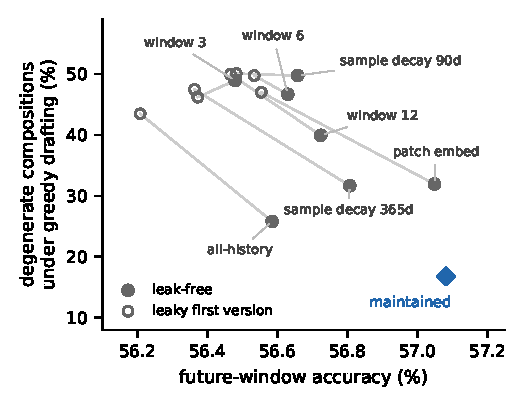
\includegraphics[width=\columnwidth]{fig_scatter.pdf}
\caption{The paper's thesis in one picture. Within the seven standard
regimes (gray), higher accuracy comes with \emph{more} degenerate
drafting (r = +0.78): along the tuning axis, accuracy ranks policies
backwards. The maintained family (blue) is better on both axes through
a shared mechanism, and within that family the two most accurate
systems buy no additional discipline. Nowhere in this design space does
an accuracy gain purchase policy safety.}
\label{fig:scatter}
\end{figure}

The degenerate-composition column, drawn as
Figure~\ref{fig:scatter}, says something different. The same
checkpoints, drafting greedily against a fixed opponent pool and scored
against the future period's realized statistics, assemble teams with no
healer, no frontline, or stacked redundant roles 43.5\% of the time when
trained the popular way and 16.8\% of the time when maintained. The gap
survives deep search. In a separate benchmark, policies trained by Monte
Carlo tree search self-play on the unmaintained and maintained value
functions draft against future-meta opponent models and produce 17.6\%
versus 9.3\% degenerate drafts (5 seeds per arm), about half the rate.
Absolute degenerate rates depend on the protocol (greedy drafting
against a fixed pool, this benchmark, and direct head-to-head play in
Section~\ref{sec:neglect} each give different levels), so we compare
arms only within a protocol.

A skeptic reading Figure~\ref{fig:scatter} might object that the most
accurate system is also the safest, so accuracy predicts policy quality
after all. Look inside the cluster: across the seven standard regimes
the correlation between accuracy and degeneracy is \textbf{+0.78}:
sixteen points of degeneracy \emph{gained} per point of accuracy. Along
the axis a practitioner actually tunes (how much history, how much
recency), accuracy ranks policies backwards. The three most accurate
standard regimes (56.48 to 56.55) all draft more degenerate teams than
the least accurate one (47.0 to 50.1\% against 43.5\%). The maintained
family sits best on both axes because era-aligned statistics happen to
help prediction and composition discipline through the same mechanism.
That shared cause is a coincidence, and it gives no selection signal. We tested whether the coincidence at least behaves
like a signal at the top of the range by running the same greedy
evaluation on the decayed-aggregate variants of
Section~\ref{sec:repair}, the two most accurate systems in the paper.
It does not: their additional +0.14pp of accuracy buys no discipline
change at all (18.9\% and 19.1\% degenerate against \maintained{}'s
16.8, a flat-to-slightly-worse move inside seed noise). Accuracy gains
do not purchase policy safety anywhere in this design space, and along
the axis practitioners tune, chasing them costs safety. Policy metrics
have to be measured directly.

We state the accuracy result the way we believe it should be framed.
These models sit roughly 6 points of edge above coin flipping, so
+0.87pp of future accuracy is a 14\% improvement in edge, and against a
fully frozen deployment the deployment-weighted edge grows from 5.13 to
6.08 points with refresh alone, a 19\% larger edge (retraining on top
reaches 6.81, Section~\ref{sec:operating}). Calling sub-point accuracy
differences small is exactly the mistake this section documents.

One control deserves mention because it quantifies a trap. A model
whose features use same-build statistics computed with knowledge of the
full build reaches 72.8\% future accuracy. That number is leakage, a
model grading games with statistics that include those games' own
outcomes, and we report it only to mark how large the trap is. The
causal version of the same idea, same-build statistics from strictly
earlier days shrunk toward the long-run prior, adds nothing over
\maintained{} (57.01 versus 57.08).

\section{The Repair: Refresh the Aggregates, Then Decay Them}
\label{sec:repair}

The best regime in Table~\ref{tab:regimes} never retrains. It refreshes
data. That invites an obvious follow-up: if recomputing aggregates helps,
should old games keep full weight inside them?

They should not. Exponentially decaying the aggregates with a 90-day
half-life, with counts shrunk toward the cumulative prior (100
pseudo-games), reaches \textbf{57.22\%} future-window accuracy against
\maintained{}'s 57.08, and the separation is seed-clean: every decayed
seed beats every cumulative seed. A 365-day half-life is a wash (57.07),
which matches the decay-curve analysis of the next section, since a
one-year half-life over a 4.5-year pool barely sharpens anything. To
guard against tuning on the test window, we re-ran the selection with a
nested cutoff several builds earlier and a pseudo-future validation
window: the 90-day family wins there too, though the shrinkage variant
within the family flips between windows, so we claim family-level
selection only.

Why does decayed refresh work where cumulative refresh nearly saturates?
A partial-refresh ablation on fixed checkpoints gives the mechanism.
Swapping which statistics get refreshed at test time, holding weights
fixed, moves future accuracy by at most $\pm$0.07pp over a three-month
horizon: the cumulative aggregates are simply too dilute for three
months of drift to move the model's inputs. Most of \maintained{}'s
advantage over all-history training is therefore baked in at training
time, by learning against statistics that tracked their own era. Decayed
aggregates change the picture because they actually move: their feature
deltas against cutoff statistics are roughly ten times larger, which is
where the extra 0.14pp lives. The ablation also assigns the credit
within the feature set, and Section~\ref{sec:signals} shows that
assignment is not the one the drift curves suggest.

Two honest wrinkles. Sharp decay stumbles on the first build after a
patch: recency-sharpened statistics describe the brand-new meta with
confidence they have not earned, and the first post-cutoff build is the
one place decay loses to the dilute cumulative pool (count shrinkage
recovers about half of the loss). Immediately after a change, priors are
safest, a point the detection section returns to. The second wrinkle is
a lesson in seed discipline that we briefly got wrong ourselves. MCTS
agents trained on the champion decayed-aggregate value function at
fifteen seeds initially looked worse-disciplined than our
cumulative-refresh agent (22.7\% degenerate compositions versus 14.5\%),
suggesting the best predictor did not train the best agent. The 14.5 was
a five-seed estimate; at fifteen seeds it is 22.0, and a direct
head-to-head between the two agents (fifteen seeds per side, 4{,}500
drafts) finds no difference in degeneracy ($z = 0.7$), synergy, or
counters. Scored on out-of-sample builds (Section~\ref{sec:neglect}),
the decayed agent drafts better-timed heroes: +0.31pp of future-meta
hero win rate ($z = 3.6$), about 1.4 points of team win probability.
\textbf{Decayed aggregates win at both levels: they predict better, and
the agents they train pick better-timed heroes with no loss of
composition discipline.} The apparent discipline gap was a seed-budget
artifact, and claims about agents need agent-level seed budgets.

This recommendation now runs in production: our public drafting tool
retrains all three models on the full corpus with 90-day-half-life
decayed aggregates on a standing monthly cadence, and serves the same
decayed statistics to the browser feature pipeline the deployed value
function was trained on.

\section{What Drifts Is Not What Matters}
\label{sec:signals}

Per-build statistics let us measure how each signal class decays.
Role-composition win rates are essentially static: correlation 0.95 with
themselves at a lag of 16 builds. Pick and ban rates are nearly as
stable. Per-hero win rate is the fastest-decaying reliable signal,
falling from 0.94 to 0.62 over the same lag. Net pairwise interaction
effects are weak but persistent, mostly within-build sampling noise, a
caution for pairwise features generally.

The natural conclusion is that hero win rate, the fastest mover, is what
refresh maintains. The partial-refresh ablation of
Section~\ref{sec:repair} tested that directly and the answer is no.
Refreshing only the hero-level aggregates while leaving the rest at the
cutoff makes the model slightly worse ($-$0.07pp against fully frozen
statistics). Refreshing only the pairwise and composition aggregates
carries the entire gain and even edges out refreshing everything. Decay
curves tell you what is changing. The ablation tells you what is worth
refreshing. Those are different questions, because refresh value tracks
what the model leans on, and this model leans on interaction statistics.
The echo from our earlier work is satisfying: in a 4{,}100-configuration
feature sweep, per-hero win rate was the one feature group with negative
marginal accuracy. The fastest-drifting signal in the game is also its
least load-bearing.

The natural follow-up is to decay each signal class at its own measured
rate, so we ran it: hero-family aggregates on a fast 90-day clock with
pair and composition aggregates on a slow 365-day one, plus the reverse
assignment as a control. Per-class clocking loses. The matched
assignment scores 57.07\% future-window accuracy, the reverse 57.15, and
both sit below uniform 90-day decay (57.19) and the shrunk champion
(57.22). The telling detail is that each cell's accuracy follows its
pair-and-composition clock and ignores its hero clock, which is the
training-time version of the
ablation's lesson: the recency gain lives in the interaction features. A
signal's decay rate and the right clock for its features are different
things, and the uniform recipe stands.

The same per-build machinery answers two questions a maintainer asks
after every patch. First, how soon can the new build's own statistics be
trusted? Patch-local hero win rates settle to within a point of their
final values after a median of about 10{,}700 games into a build (75th
percentile 12{,}200), a threshold Section~\ref{sec:detect} will place
next to the detector's latency. Within tiers the order is low (6{,}500
of that tier's games), high (7{,}800), then mid (8{,}700); slice counts
flatter this metric mechanically, so they rank tiers against each other
and are not comparable with the pooled figure.
Meta stability itself is tier-ordered and measurable, while composition
structure is stable at every tier. Second, does drift move which
compositions never get played? Barely: the never-fielded composition set
has a consecutive-build Jaccard similarity of 0.81, and past the first
few hundred thousand games of corpus it is volume-driven rather than
meta-driven. That is quietly a durability result for our earlier paper,
whose synthetic-augmentation method targets exactly that set: the
targets would have been essentially the same in any era, so the method
does not need re-derivation each patch.

\begin{figure}[t]
\centering
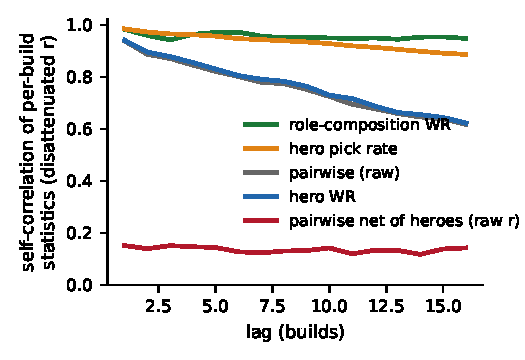
\includegraphics[width=\columnwidth]{fig_decay.pdf}
\caption{Signal-class decay. Self-correlation of per-build aggregate
statistics as a function of build lag. Role-composition structure is
static; per-hero win rate decays fastest. Section~\ref{sec:signals}
shows decay speed does not predict refresh value.}
\label{fig:decay}
\end{figure}

\section{Detecting Balance Changes from Outcomes Alone}
\label{sec:detect}

A maintenance policy needs a trigger. The developer's patch notes
provide ground truth: we scripted 40 mapped patches and five documented
no-change builds, covering all 27 boundaries large enough to be
detectable in principle. The detector tests each hero's win rate across
each build boundary and keeps the shifts that survive false-discovery-rate
correction. Against the ground truth, \textbf{0.79 of its hero flags}
(46 of 58) name a hero the notes changed, and at the level that matters
for maintenance, \textbf{16 of the 17 boundaries where it fires} carry
documented balance changes (precision 0.94): when outcomes move, the
developer almost always shipped a change. The same test on pick and ban
rates behaves differently, with hero-level recall 0.68 but precision
0.32. That detector picks up the community noticing, which spills across
build boundaries and fires on hype as readily as on tuning. Outcome
statistics detect the patch; behavior statistics detect the reaction.

The heroes the detector confirms first cross significance, in a
sequential version of the same test, a median of 7{,}000 games into a
build (10{,}200 under a sequential probability ratio test). In wall-clock
terms that is under a week at our live inflow of roughly fifteen
thousand new ranked games per week, which is how a practitioner should
read it: a balance change is statistically confirmable from outcomes
alone within about a week of shipping. The latency number also lands
next to another one: the point at which a build's own statistics become
trustworthy to within a point of their settled values is a median of
10{,}700 games (75th percentile 12{,}200). Detection and repair arrive
on the same timescale. By the time you can prove something changed, the data to
respond with already exists.

The loop closes in simulation. Adding a detector-triggered arm to the
deployment replay of Section~\ref{sec:operating}, with the refresh
honestly lagged by each detection's own latency, matches blind
every-build refreshing to within \textbf{0.013pp} while performing 14
refreshes instead of 35. Latency itself is nearly free: pessimistically
lagging every refresh by the full median detection delay costs 0.015pp
total. Detection and repair close into a single working loop.

None of this depends on our particular threshold. Sweeping the
detector's false-discovery level across two orders of magnitude moves
hero-level precision from 0.90 at the strictest setting to 0.45 at the
loosest,
while every operating point on the deployment replay lands within
0.03pp of every other, all of them recovering most of the gap between
leaving the same model's statistics unrefreshed (+1.06pp regret) and
refreshing them every build (+0.73pp). (Table~\ref{tab:regret}'s larger
never-maintain row, +1.68, is a different condition: there the model is
also \emph{trained} on frozen-statistics features; the sweep isolates
the refresh decision on a fixed model.) The trigger can be tuned for
precision or for coverage and the maintenance outcome barely moves,
which is what a practitioner wants from a component they will not be
watching. At the boundary level, the unit that matters for maintenance,
our threshold fires on 16 of the 21 boundaries with true balance
changes and stays silent on 5 of the 6 documented no-change boundaries.
The misses include two roster-wide cleanup patches that list 64 and 88
heroes but consist mostly of bug fixes and interface changes (one lists
60 separate fixes).
(Per-hero recall reads much lower, 0.06 at our setting, because the
ground truth counts every individual hero change in the notes, most of
which are singly too small to detect. The full sweep is in the released
artifacts.)

\section{The Cost of Neglect, Measured Head-to-Head}
\label{sec:neglect}

Accuracy comparisons leave a fair question open: does any of this matter
when policies actually play? We answer with direct competition. The
\maintained{} agent drafts against three unmaintained agents, 2{,}000
drafts per matchup (five seeds per side, all twenty-five seed pairings,
both first-pick orderings, maps and tiers stratified). The design
separates two things. \stalefour{} shares \maintained{}'s training
cutoff, so the first matchup prices maintenance itself: training against
era-aligned statistics plus three months of statistics refresh.
\staleone{} and \staletwo{} keep the unmaintained recipe fixed and move
the cutoff back one and two years, so differences between the rows
price staleness alone. The deployment replay of
Section~\ref{sec:operating} splits the first quantity at the accuracy
level: of the 0.95pp that maintenance recovers there, about two thirds
comes from the training recipe (1.68 versus 1.06pp regret without any
refresh) and one third from the refresh itself (1.06 versus 0.73).

Scoring these games is where evaluation bit us twice, so we state the
protocol precisely. No learned judge decides anything. Each terminal
draft is scored against the \emph{realized outcomes of the future}: the
average future-meta win rate of the heroes each side picked, the
synergy of each side's pairs and its counters against the other side's
heroes (pair and matchup win rates beyond what the heroes' own rates
predict), and the rule-based degenerate-composition flag. The future is
298{,}428 ranked games from five builds, May through September 2026
(2.55.16.97039 and four 2.55.17 builds), that no agent's statistics
touch. Our first version of this protocol scored against all seven
post-cutoff builds, and six of those also fed the maintained agent's
drafting statistics. That overlap tripled the four-month synergy gap
(+0.76 against +0.23 out of sample) and hid a real difference between
the two maintained variants (Section~\ref{sec:repair}). Inference
charges seed variance properly, with crossed random effects for the two
seed identities.

\begin{table}[t]
\caption{Cost of neglect, scored on out-of-sample builds. Deficit: the
unmaintained agent's shortfall in future-meta hero win rate (pp,
crossed-seed random effects). Net: the team win-probability gap implied
by hero, synergy, and counter scores together, with weights fitted on
held-out real games (mean of two cross-fitting splits; $z \geq 2.0$ in
every split). The last row replaces \maintained{} with a maintained agent
trained on exactly \staletwo{}'s data volume.}
\label{tab:dose}
\centering
\footnotesize
\setlength{\tabcolsep}{4pt}
\begin{tabular}{lccc}
\toprule
Opponent & Deficit (pp) & $z$ & Net (pp) \\
\midrule
\stalefour{} & $+0.66 \pm 0.15$ & 4.3 & +2.7 \\
\staleone{} & $+0.56 \pm 0.21$ & 2.7 & +2.5 \\
\staletwo{} & $+1.10 \pm 0.17$ & 6.5 & +4.1 \\
\staletwo{}, volume-matched & $+1.00 \pm 0.20$ & 5.0 & +3.7 \\
\bottomrule
\end{tabular}
\end{table}

Table~\ref{tab:dose} is the headline. Maintenance is worth +0.66pp of
future-meta hero win rate against an unmaintained agent with the same
training data, and the fifteen-seed replication of that matchup (4{,}500
drafts) gives +0.69 $\pm$ 0.10 ($z = 7.0$). An extra year of staleness
adds nothing measurable (+0.56). A second year adds about half a point:
the two-year deficit is +1.10, and its rise over the first two rows is
$+0.49 \pm 0.21$. Because our corpus grows over time, the two-year agent
also trained on fewer games, so we ran the control: a maintained agent
trained on exactly the \staletwo{} row count keeps +1.00pp, 91\% of the
edge. Volume explains less than a tenth of the two-year gap.

Hero win rate is a per-hero quantity, so we also ask what the three
realized-outcome metrics add up to. Splitting the future games in half,
we compute the statistics on one half and fit a three-term logistic
model of real results on the other: hero win rate, synergy, and counter
scores all predict wins, with hero win rate dominant ($z \approx 50$,
against 12 for counters and 8 for synergy). Applied to the head-to-head
drafts, those weights put the maintained agent 2.5 to 4.1 points of
team win probability ahead (the Net column).

The metrics also show what does not decay. Out of sample, the synergy
gap is small at every level (+0.23, +0.25, and +0.07 at two years;
+0.18 in the fifteen-seed replication), so synergy knowledge keeps for
years. Counters run
the other way. Unmaintained agents counter the maintained agent's picks
slightly better, significantly so at two years ($-0.56 \pm 0.13$,
$z = -4.4$) and in the fifteen-seed replication ($-0.31 \pm 0.08$). The
gap survives changes to the metric: a counter score computed on the
log-odds scale, or with the trend on hero strength removed, gives the
same gaps. Weighted by how much each metric predicts real wins, the
counter edge gives back about a sixth of the timing deficit. The
two-year deficit is therefore almost all hero timing, the drift class
Section~\ref{sec:signals} found fastest, showing up end-to-end in an
agent.

The maintained agent also drafts fewer degenerate compositions. At full
power (fifteen seeds per side, 4{,}500 head-to-head drafts) the rates
are 22.0\% maintained versus 36.9\% unmaintained, a paired difference
of 15.0pp ($\pm 6.7$ under crossed seed effects, $z = 2.2$). Across the
three five-seed matchups the unmaintained side's rate does not rise
with staleness (35\%, 28\%, and 28\%), and the maintained side's
advantage (21, 8, and 8 points) is directional in each matchup alone
($|z| \leq 1.8$). Composition discipline looks durable, and the training
recipe is what sets it.

\section{Evaluators Drift Too}
\label{sec:vintage}

The obvious way to score the head-to-heads was the consensus of our
win-probability models, the same panel that adjudicated our earlier
tournament. We did that first, got +0.8pp for the maintained side, and
then noticed the number was unidentified: those judges are trained on a
snapshot that includes the future period, so they share the maintained
agent's information advantage by construction. The fix produced a
finding.

We trained naive-feature judges (hero identities, map, and tier only, no
aggregate statistics) in two corpus families and scored the same
2{,}000 \maintained{}-versus-\stalefour{} drafts with every judge. Six
ranked-play judges span early 2022 through the cutoff build, each
trained on the 314{,}761 most recent games before its cutoff, except the
earliest (2022Q1), which had only 158{,}709 games to learn from. Four Quick-Match judges (2021, 2022, 2024, 2026,
on their natural pools of 29K--129K games) come from a different game
mode entirely: Quick Match has no draft phase, teams are assembled by
the matchmaker, so these judges' training data contains no drafts and
cannot share either agent's training distribution. The ranked verdict
rises with judge era: 0.469 and 0.461 (two 2022 judges), 0.493 (2023),
and 0.495 to 0.513 for 2024 through 2026. The Quick-Match family
replicates the pattern from its disjoint corpus: 0.434 (2021) and 0.416
(2022), then 0.494 (2024) and 0.508 (2026). Judge seeds move these
scores by about 0.011, so we read everything within that of 0.50 as
parity. \textbf{Every judge trained before 2023, in either family,
declares the unmaintained agent the winner of a 2026 contest; from 2023
on, judges call it roughly even.} None of them can credit the
maintained agent's realized edge, since none saw the scoring period,
but the old ones confidently invert it. Nothing is wrong with the old
judges except their era: what separates these two agents is largely
current-meta knowledge, which an old judge cannot see and mis-scores.
And because the Quick-Match family moves from 0.416 to 0.508 with the
mode held fixed, the reversal tracks the judge's era within a single
corpus family.

\begin{figure}[t]
\centering
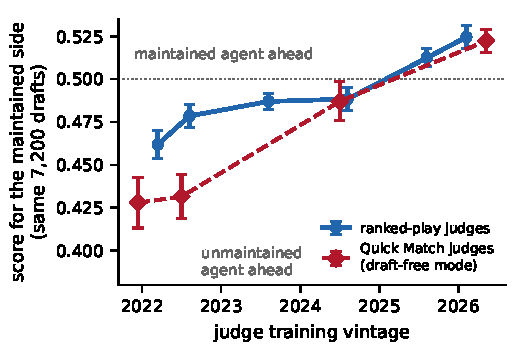
\includegraphics[width=\columnwidth]{fig_vintage.pdf}
\caption{The vintage matrix. Score assigned to the maintained side of
the same 2{,}000 drafts by win-probability judges trained at different
historical vintages. Old judges reverse the verdict; judges from 2023
on score the contest roughly even. Diamonds: judges trained on Quick Match, a
mode with no draft phase (teams are matchmade), so their training data
contains no drafts and is disjoint from both agents'; the family
replicates the era trend, isolating era from corpus.}
\label{fig:vintage}
\end{figure}

Yet the oldest and newest Quick-Match judges (2021 and 2026) both
reproduce our earlier tournament's ordering at rank correlation 0.92.
That is the reconciliation, and it is useful: contests
decided by composition structure are stable across eras, because
structure barely drifts (Section~\ref{sec:signals}); contests decided by
meta timing are exactly where judge vintage matters most. The practical
consequence for anyone evaluating agents in a drifting domain: a learned
judge is a model of a meta and ages like one; date your judges, report
them as a matrix, and put your headline on realized outcomes.

\section{The Opponent Model Drifts on Its Own Clock}
\label{sec:opponent}

Everything above maintains the value function. A deployed drafter also
carries a behavioral model of its opponent (the next-pick predictor that
guides search rollouts), and player behavior drifts on a different
schedule than balance. We tested five opponent-model pools on 1.84
million next-pick samples from the future builds
(Table~\ref{tab:gdpools}).

\begin{table}[t]
\caption{Opponent-model pools evaluated on 1.84M future next-pick
samples. Top-1/top-5 are future-window next-pick accuracies.}
\label{tab:gdpools}
\centering
\small
\setlength{\tabcolsep}{4pt}
\begin{tabular}{lcc}
\toprule
Pool & Top-1 \% & Top-5 \% \\
\midrule
future oracle (trained on test period) & 13.09 & 40.39 \\
30-day rolling window & \textbf{11.83} & \textbf{36.98} \\
\leakyfrozen{} (statistics saw the future) & 11.71 & 36.31 \\
6-build recency window & 11.64 & 36.91 \\
causal cutoff (all history to cutoff) & 11.08 & 34.47 \\
\bottomrule
\end{tabular}
\end{table}

Three gaps decompose the table. Behavioral drift costs the deployable
cutoff model 0.63pp of top-1 against the leaky reference. Recency buys
most of it back (+0.56pp for a 6-build window), and a 30-day rolling
window buys more than all of it back (+0.75pp), beating even the leaky
pool whose statistics saw the future. The rolling window then decays
across the later test builds (13.12 on the first down to 10.61 as its
window goes stale), which is the point: behavior wants
\emph{continuous} refresh. Player adaptation, unlike balance, never
ships in discrete builds.

We had set a materiality trigger for this arm in advance: if
behavioral drift cost at least 1.0pp of top-1, or if swapping opponent
pools moved the maintained value function's policy cells by at least
3pp, we would retrain the full MCTS pipeline on refreshed opponents.
Neither condition was met: 0.63pp against the 1.0pp accuracy threshold,
and movements of 2.9pp of healer rate and 2.7pp of degenerate rate
against the 3.0pp threshold, in the direction of slightly cleaner
compositions under the causal pool. (The all-history value function,
which the trigger did not cover, moved more: 5.8pp of healer rate and
3.5pp of degenerate rate.) By rule the expensive arm did not run.
Honoring a no-go set in advance is as much a part of the method as the
runs we did make.

\section{The Operating Policy}
\label{sec:operating}

We replay a 2.8-year deployment forward across 36 builds, starting from
roughly 640{,}000 games of history, and score every maintenance policy
by games-weighted accuracy and by regret against an oracle that retrains
after every build (Table~\ref{tab:regret}).

\begin{table}[t]
\caption{Deployment replay over 2.8 years (deployment-weighted accuracy;
regret versus retraining every build).}
\label{tab:regret}
\centering
\footnotesize
\setlength{\tabcolsep}{4pt}
\begin{tabular}{lccc}
\toprule
Policy & Retrains & Refreshes & Regret (pp) \\
\midrule
oracle: retrain every build & 35 & 35 & 0.000 \\
never retrain, frozen aggregates & 0 & 0 & +1.682 \\
never retrain, refresh per build & 0 & 35 & +0.730 \\
refresh + retrain every 3 builds & 11 & 35 & +0.029 \\
refresh + warm-start finetune & 11 & 35 & +0.089 \\
detector-triggered refresh only & 0 & 14 & +0.743 \\
\bottomrule
\end{tabular}
\end{table}

The table supports a plain reading. Doing nothing costs 1.68pp over the
deployment. Refresh alone recovers more than half of that without
touching the weights. Once statistics are fresh, any reasonable
retraining style, full or warm-start, lands within 0.1pp of the oracle,
so the retraining schedule becomes an operational convenience. And the detector-triggered row shows the trigger
works outside the lab framing: fourteen refreshes, honestly lagged,
match thirty-five blind ones.

The trigger's design matters for domains without a patch calendar. We
tested whether patch timing could be inferred from match data alone: a
multi-scale changepoint detector over daily hero pick, ban, and win
rates, tuned on pre-2025 boundaries and evaluated held out, recovers
only the largest patches (day-level timing when it fires, but held-out
precision 0.18 at recall 0.27, and most boundaries score below ambient
weekly variation). Blind detection cannot reconstruct the event
calendar, and only a labeled domain like this one can measure that
failure; a practitioner in an unlabeled domain would have no way to know
which changes they were missing. Our trigger needs much less than the
patch calendar. It needs version identifiers, which almost every
deployed system logs, and it fires on the magnitude of the outcome shift
between versions whatever the cause, with no patch notes or labels. That
is the property that transfers to domains where changes arrive
unannounced.

Assembled with Section~\ref{sec:opponent}, the operating policy has
three speeds: feature aggregates every build or on detector fire,
opponent model on a rolling month, value model whenever convenient. This
is what our production deployment now runs.

\section{A Prospective Test, Pre-Registered}
\label{sec:prospective}

Every result above is retrospective: the cutoff was chosen, then the
future window was scored. Retrospective drift studies can be tuned, even
accidentally, to the future they hold out. So before submission we
registered three forward claims on OSF (\preregdate{};
\prereglink{}), with the analysis code frozen by commit hash: (1) the
outcome-shift detector, decision rule untouched, fires on new builds
whose patch notes contain sizable balance changes and stays silent on
no-change builds (builds whose changes are only bug fixes or
individually minor tweaks are reported descriptively and adjudicate
nothing; retrospectively they are exactly where the detector misses);
(2) the existing head-to-head drafts, rescored with the out-of-sample
protocol of Section~\ref{sec:neglect} against the new builds' realized
statistics, keep a positive maintained advantage in future-meta hero
win rate (both agents and all drafts predate those builds entirely, so
nothing in this claim can be tuned); (3) every production refresh event
is logged and reported against the detector's fires. The claims cover
only builds that ship after the registration date. The builds between
our snapshot and the registration (2.55.16.97039 and the four 2.55.17
builds) already serve as the out-of-sample scoring set of
Section~\ref{sec:neglect}, so they are excluded. On power: new ranked
games arrive at roughly fifteen thousand per week, so a new build
reaches detector-decidable volume in under two weeks. Sizable builds have
historically shipped every six to nine weeks, so a six-month review
window should contain three or four. We report every outcome, however
many builds that turns out to be.
% [PROSPECTIVE RESULTS: filled at the revision analysis date, per
% paper/drift/PREREG_FORWARD.md. Submission does NOT wait for this
% section's results.]

\section{Related Work}
\label{sec:related}

Concept drift and dataset shift have a large literature, most of it
classifier-centric: detect distributional change, adapt the model,
measure accuracy~\cite{quinonero2009dataset,gama2014survey,lu2018learning}.
The canonical detectors monitor a supervised error stream (DDM tracks
error-rate inflation~\cite{gama2004ddm}; ADWIN maintains adaptive
windows over it~\cite{bifet2007adwin}), and adaptation means retraining
or reweighting the classifier. Our setting breaks both halves of that
recipe: the quantity that degrades (policy behavior) is not the quantity
those detectors watch (accuracy), and the cheapest effective adaptation
touches no weights at all. Change-point detection supplies the standard
machinery~\cite{aminikhanghahi2017survey}; our detector is deliberately
plain, and the contribution is the ground truth we score it against
(developer patch notes) and the loop it closes. Our contribution to the
drift conversation itself is the object being damaged. In a
combinatorial decision system, sub-point accuracy movement coexists with
multiples of policy-level failure, so drift monitoring that watches
accuracy watches the wrong gauge.

Continual and non-stationary reinforcement learning study policies that
must keep learning as the environment changes, spanning formal
treatments of non-stationary MDPs~\cite{padakandla2021survey} and the
continual-RL research agenda~\cite{khetarpal2022continual}, with
catastrophic forgetting as a central obstacle when the learner must
retain old competence~\cite{kirkpatrick2017ewc}. That literature mostly
asks how to keep \emph{training}; the deployed case we study inverts the
question: the policy is fixed between maintenance events, and the
decision is when and what to touch. Our finding that decayed aggregates
beat retraining is a statement about that regime. It leaves
continual-learning algorithms untested, and the two are complementary: a
continual learner still needs the trigger, the evaluator hygiene, and
the fresh statistics this paper prices. On the operations side, the
engineering literature has long flagged data dependencies and feature
freshness as the dominant maintenance surface of deployed
ML~\cite{sculley2015debt}, production-readiness rubrics score exactly
the monitoring loop we close~\cite{breck2017mltest}, data-validation
systems treat statistics staleness as a first-class
failure~\cite{polyzotis2019data}, and interview studies of practitioners
report retraining cadence as a recurring open
question~\cite{shankar2022operationalizing}; our results give those
observations teeth, with a measured decomposition of how much refresh
and retraining each buy and a mechanism for why the data side dominates
here. In games, drafting has been treated as a prediction and
recommendation problem, from pick prediction in Dota
2~\cite{summerville2016draft} to team-aware hero
recommendation~\cite{chen2018art} and personalized draft
recommendation~\cite{draftrec}, and balance evaluation has its own
methods~\cite{jaffe2012balance}; to our knowledge none of this work
measures maintenance policies against a patch-note ground truth or
prices staleness in head-to-head play. Offline reinforcement learning
under non-stationarity is usually posed as a training-time
problem~\cite{levine2020offline}; here the policy is fixed and the world
moves, which is the deployed case. Within our own series, this paper is
the time-axis companion to our draft-policy paper~\cite{paper1}: the
same decomposition, the same policy-first evaluation discipline, pointed
at drift. Player-skill drift, the third timescale, is deliberately out of
scope here and is the subject of a companion study of personalization.

\section{Limitations}
\label{sec:limits}

Everything here is one game and one major patch, a scoping we accept
deliberately: it buys 45 within-rules balance builds with a fixed hero
pool, at the cost of external validity we will need to earn elsewhere.
The judge-free protocol rests on realized future outcomes at the level
of hero, pair, and matchup statistics, which are marginal quantities; we
mitigate by triangulating the metrics, by combining them with weights
fitted on held-out real games (a three-parameter model, far simpler than
any judge), and by reporting learned judges only through the vintage
matrix. At the agent level we price maintenance as a package: the
training recipe and the statistics refresh come together, and only the
deployment replay separates them (about two thirds recipe, one third
refresh, at the accuracy level). An agent-level split would need an
agent trained with the maintained recipe and then frozen, which we did
not build. The staleness gradient has three points, enough for shape
claims at the resolution we make them and not more. Finally, our
scoring protocols went wrong twice before they went right. The first
used an evaluator panel that shared the maintained agent's vintage, and
catching that confound produced Section~\ref{sec:vintage}. The second
scored against future statistics that overlapped the maintained
agent's own inputs, and moving to builds no agent had touched shrank
the synergy results while leaving the timing results intact. Each
correction made the results smaller and the claims stronger. We think
that trade is the right advertisement for the methods.

\section{Conclusion}

An unmaintained draft policy picks heroes that win about 0.7 points
less often in the future meta, roughly 2.7 points of team win
probability, and the gap passes a full point after two years. The loss
is invisible to accuracy and to any evaluator old enough to share the
neglect. The repair is unglamorous: keep the feature aggregates fresh,
decay them, let an outcome-shift detector time the work, and retrain
whenever it is cheap, since retraining adds little once the statistics
are fresh. The pattern we keep finding, including in our own analysis
pipeline, is that differences which look decisive at one level vanish
or invert at another. Maintenance is a policy decision. Evaluate it
like one.

\ifanonymous
\section*{AI Disclosure}
Portions of this manuscript's text were drafted and edited with Claude
(Anthropic)~\cite{claude}; all experiments, analyses, and claims were
designed, verified, and approved by the authors.
\else
\section*{Acknowledgments}
We thank Heroes Profile for API access to replay data (a paid service,
and an open-source project we are glad to support), and the NGS
community for organized-league data used in our earlier work. Portions
of this manuscript's text were drafted and edited with Claude
(Anthropic)~\cite{claude}; all experiments, analyses, and claims were
designed, verified, and approved by the authors.
\fi

\begin{thebibliography}{12}
\bibitem{paper1} \ifanonymous Anonymous authors\else M.~Segan,
E.~Pysher, J.~Frankel, and H.~Lipson\fi, ``Diagnosing and repairing
out-of-distribution failure in MOBA draft policies,'' under review,
2026.
\bibitem{quinonero2009dataset} J.~Qui\~nonero-Candela, M.~Sugiyama,
A.~Schwaighofer, and N.~D. Lawrence, Eds., \emph{Dataset Shift in
Machine Learning}. MIT Press, 2009.
\bibitem{gama2014survey} J.~Gama, I.~\v{Z}liobait\.{e}, A.~Bifet,
M.~Pechenizkiy, and A.~Bouchachia, ``A survey on concept drift
adaptation,'' \emph{ACM Computing Surveys}, vol.~46, no.~4, 2014.
\bibitem{lu2018learning} J.~Lu, A.~Liu, F.~Dong, F.~Gu, J.~Gama, and
G.~Zhang, ``Learning under concept drift: A review,'' \emph{IEEE
Transactions on Knowledge and Data Engineering}, vol.~31, no.~12,
pp.~2346--2363, 2019.
\bibitem{aminikhanghahi2017survey} S.~Aminikhanghahi and D.~J. Cook,
``A survey of methods for time series change point detection,''
\emph{Knowledge and Information Systems}, vol.~51, no.~2, 2017.
\bibitem{gama2004ddm} J.~Gama, P.~Medas, G.~Castillo, and P.~Rodrigues,
``Learning with drift detection,'' in \emph{Brazilian Symposium on
Artificial Intelligence (SBIA)}, 2004.
\bibitem{bifet2007adwin} A.~Bifet and R.~Gavald\`a, ``Learning from
time-changing data with adaptive windowing,'' in \emph{Proc. SIAM
International Conference on Data Mining}, 2007.
\bibitem{padakandla2021survey} S.~Padakandla, ``A survey of
reinforcement learning algorithms for dynamically varying
environments,'' \emph{ACM Computing Surveys}, vol.~54, no.~6, 2021.
\bibitem{khetarpal2022continual} K.~Khetarpal, M.~Riemer, I.~Rish, and
D.~Precup, ``Towards continual reinforcement learning: A review and
perspectives,'' \emph{Journal of Artificial Intelligence Research},
vol.~75, pp.~1401--1476, 2022.
\bibitem{kirkpatrick2017ewc} J.~Kirkpatrick \emph{et al.}, ``Overcoming
catastrophic forgetting in neural networks,'' \emph{Proceedings of the
National Academy of Sciences}, vol.~114, no.~13, pp.~3521--3526, 2017.
\bibitem{sculley2015debt} D.~Sculley, G.~Holt, D.~Golovin, E.~Davydov,
T.~Phillips, D.~Ebner, V.~Chaudhary, M.~Young, J.-F. Crespo, and
D.~Dennison, ``Hidden technical debt in machine learning systems,'' in
\emph{Advances in Neural Information Processing Systems}, 2015.
\bibitem{breck2017mltest} E.~Breck, S.~Cai, E.~Nielsen, M.~Salib, and
D.~Sculley, ``The ML test score: A rubric for ML production readiness
and technical debt reduction,'' in \emph{IEEE International Conference
on Big Data}, 2017.
\bibitem{polyzotis2019data} N.~Polyzotis, M.~Zinkevich, S.~Roy,
E.~Breck, and S.~Whang, ``Data validation for machine learning,'' in
\emph{Proc. Machine Learning and Systems (MLSys)}, 2019.
\bibitem{shankar2022operationalizing} S.~Shankar, R.~Garcia, J.~M.
Hellerstein, and A.~G. Parameswaran, ``Operationalizing machine
learning: An interview study,'' arXiv:2209.09125, 2022.
\bibitem{summerville2016draft} A.~Summerville, M.~Cook, and
B.~Steenhuisen, ``Draft-analysis of the Ancients: Predicting draft
picks in DotA 2 using machine learning,'' in \emph{AIIDE Workshop on
Experimental AI in Games}, 2016.
\bibitem{chen2018art} Z.~Chen, T.-H.~D. Nguyen, Y.~Xu, C.~Amato,
S.~Cooper, Y.~Sun, and M.~S. El-Nasr, ``The art of drafting: A
team-oriented hero recommendation system for multiplayer online battle
arena games,'' in \emph{Proc.\ ACM Conference on Recommender Systems
(RecSys)}, 2018.
\bibitem{draftrec} H.~Lee et al., ``DraftRec: Personalized draft
recommendation for winning in multi-player online battle arena games,''
in \emph{Proc.\ ACM Web Conference (WWW)}, 2022.
\bibitem{jaffe2012balance} A.~Jaffe, A.~Miller, E.~Andersen, Y.-E.
Liu, A.~Karlin, and Z.~Popovi\'c, ``Evaluating competitive game balance
with restricted play,'' in \emph{Proc.\ AAAI Conference on Artificial
Intelligence and Interactive Digital Entertainment (AIIDE)}, 2012.
\bibitem{levine2020offline} S.~Levine, A.~Kumar, G.~Tucker, and J.~Fu,
``Offline reinforcement learning: Tutorial, review, and perspectives on
open problems,'' arXiv:2005.01643, 2020.
\bibitem{claude} Anthropic, ``Claude (Fable 5),'' large language model,
2026.
\end{thebibliography}

\end{document}
